\documentclass[12pt]{article} % use larger type; default would be 10pt
\usepackage[utf8]{inputenc} % set input encoding (not needed with XeLaTeX)
%%% PAGE DIMENSIONS
\usepackage{geometry} % to change the page dimensions
\geometry{a4paper} % or letterpaper (US) or a5paper or....
\geometry{margin=2cm} % for example, change the margins to 2 inches all round
% \geometry{landscape} % set up the page for landscape
%   read geometry.pdf for detailed page layout information
\usepackage{graphicx} % support the \includegraphics command and options
\graphicspath{ {./images/} }
% \usepackage[parfill]{parskip} % Activate to begin paragraphs with an empty line rather than an indent
%%% PACKAGES
\usepackage{booktabs} % for much better looking tables
\usepackage{array} % for better arrays (eg matrices) in maths
\usepackage{paralist} % very flexible & customisable lists (eg. enumerate/itemize, etc.)
\usepackage{verbatim} % adds environment for commenting out blocks of text & for better verbatim
\usepackage{subfig} % make it possible to include more than one captioned figure/table in a single float
% These packages are all incorporated in the memoir class to one degree or another...
%%% HEADERS & FOOTERS
\usepackage{fancyhdr} % This should be set AFTER setting up the page geometry
\pagestyle{fancy} % options: empty , plain , fancy
\renewcommand{\headrulewidth}{0pt} % customise the layout...
\lhead{}\chead{}\rhead{}
\lfoot{}\cfoot{\thepage}\rfoot{}
%%% SECTION TITLE APPEARANCE
\usepackage{sectsty}
\allsectionsfont{\sffamily\mdseries\upshape} % (See the fntguide.pdf for font help)
% (This matches ConTeXt defaults)
%%% ToC (table of contents) APPEARANCE
\usepackage[nottoc,notlof,notlot]{tocbibind} % Put the bibliography in the ToC
\usepackage[titles,subfigure]{tocloft} % Alter the style of the Table of Contents
\renewcommand{\cftsecfont}{\rmfamily\mdseries\upshape}
\renewcommand{\cftsecpagefont}{\rmfamily\mdseries\upshape} % No bold!

% Better inline directory listings
\usepackage{xcolor}
\definecolor{light-gray}{gray}{0.95}
\newcommand{\code}[1]{\colorbox{light-gray}{\texttt{#1}}}

\usepackage{parskip}


%%% END Article customizations

%%% The "real" document content comes below...

\title{Report for Seminar Assignment 1}
\author{Luka Uranič, Nejc Uršič}
\date{19.11.2022} % Activate to display a given date or no date (if empty),
         % otherwise the current date is printed 

\begin{document}
\maketitle
\begin{center}
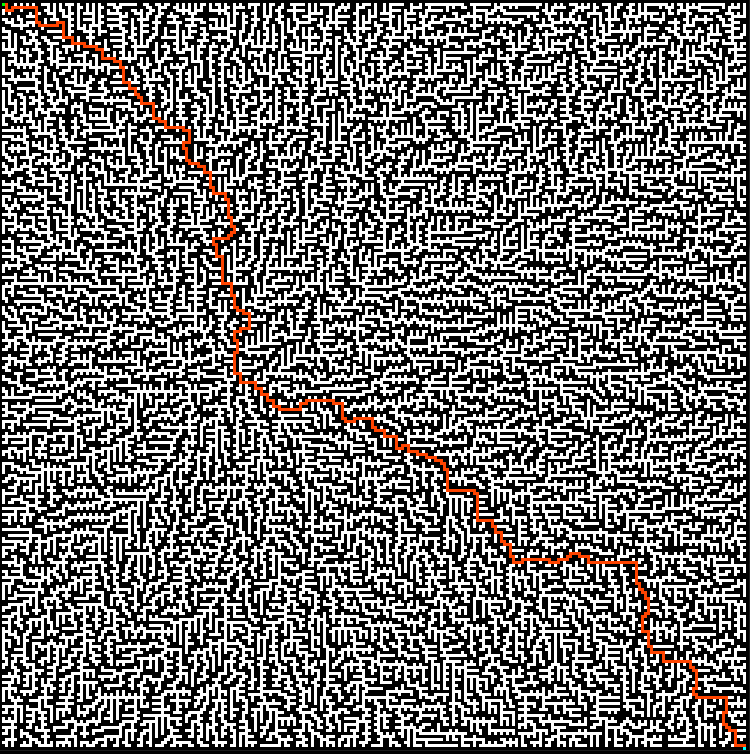
\includegraphics[scale=.75]{bigMaze}
\end{center}

\section{Introduction}
In the first seminar assignment, out goal was to use genetic algorithm to find a path out of a maze,
represented as a vector of strings, where \# character represents a wall, . represents empty space, and
S and E represent the starting and ending points.
You can move through the maze in four directions, left, right, up, and down. Out task was to create a function that will be able to find path
 as short as possible out of any maze represented in such a way.

\section{Task 1-  Representation}
Maze is represented as a vector/array of Strings and then gets transformed into one dimensional integer array that represents the maze matrix. Where
\# is stored as -1, . as 0, S as 1, E as 2 and T as 3. Start, end and positions of tressures are stored as Vec2 object which is a vector with two int values (maze coordinates).

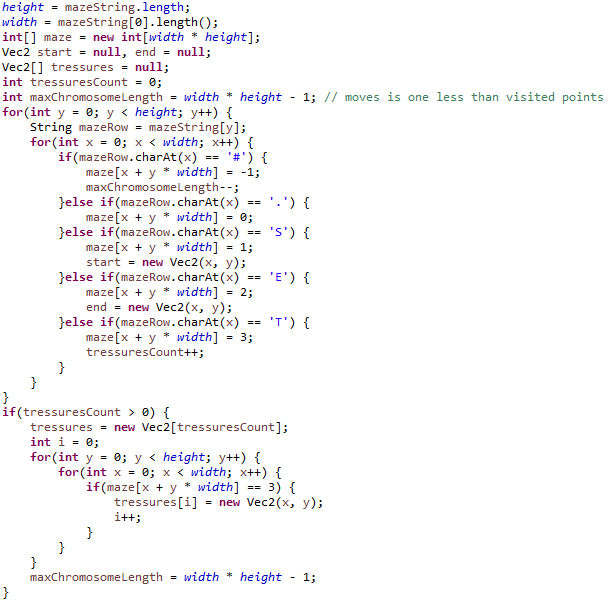
\includegraphics{stringToData}

Solution is a sequence of moves to get from start position to end position (example: LUDUULDR). The solution representation is array of Integers where 0 means left, 1 means right, 2 means up and 3 means down.

Fitness function calculates the fitness of a Chromosome. Chromosomes with a better fitness are more likely to survive and reproduce. Fitness function maximum is when distance to end position is 0, never goes through walls, the path is shortest possible and all thresures are on the path.

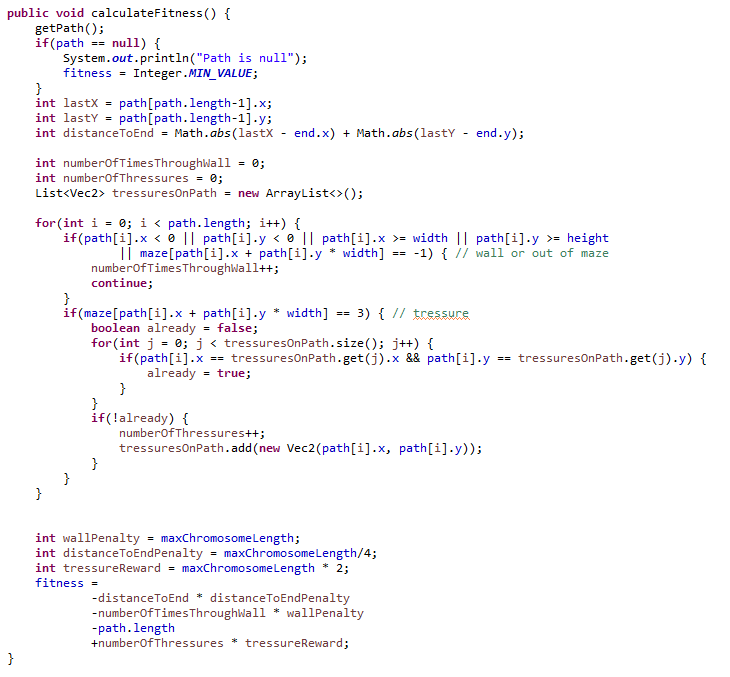
\includegraphics[scale=1]{fitnessFunction}



\section{Task 2,3 - Selection, crossover, mutations, initial population}
Our implementation of genetic algorithm (for solving maze problem):

\subsection{Selection}
\subsubsection{Random selection}
Randomly selects two parents (fitness doesn't matter):

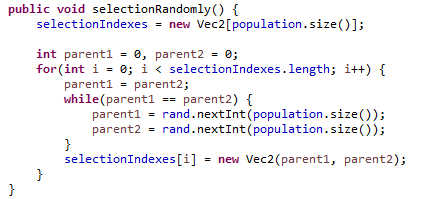
\includegraphics[scale=1]{randomSelection}

\subsubsection{Linearly biased selection}
Randomly selects two parents, but parents with greater fitness have a bigger probabiliy to get selected (linearly biased distrobution):

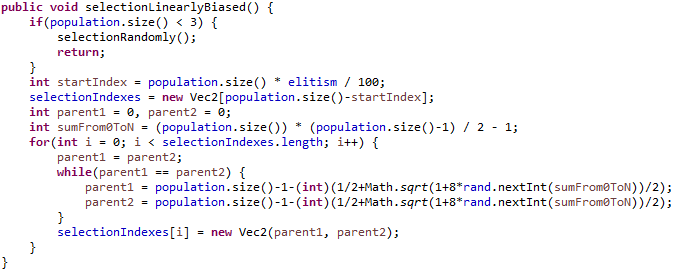
\includegraphics[scale=1]{linearSelection}


\subsubsection{Higher order biased selection}
Randomly selects two parents, but parents with greater fitness have a bigger probabiliy to get selected (higer order biased distrobution). We didn't implement it, but different probability distributions might improve the algorithm.

\subsection{Crossover}
\subsubsection{Pick a random parent}
Picks a random parent to become a new child:

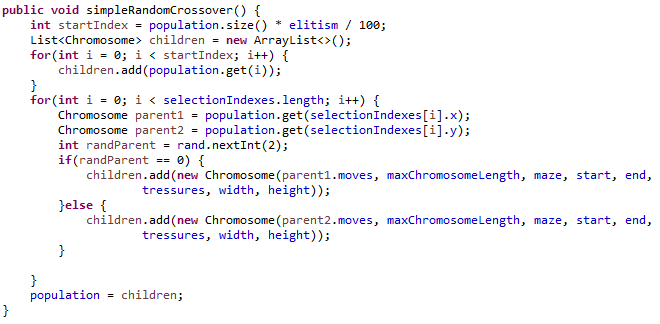
\includegraphics[scale=1]{pickARandomParentCrossover}


\subsubsection{Intersections crossover}
Go through all intersections between two parents paths than select a random intersection and build a new path like this: randomly select a path to the
intersection from one of the parents, randomly select the path after intersection from one of the parents. With this method you have to be careful, 
because not all the lengths of path are the same so you can easily get unexpected results. We implemented this method, but was computationaly to slow 
and didn't work better than the randomly pick a parent so we decided to use that one insted.

\subsection{Mutations}
\subsubsection{Random mutation}
Randomly mutate a single move along the path.

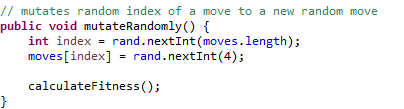
\includegraphics[scale=1]{randomMutation}

\subsubsection{Random mutation with path correction}
Randomly mutate a single move along the path and then corrects all the moves afterwards so that they don't go into walls of the maze. For better
algorithm performance you should also make back moves less likely, so that a bigger part of a maze is searched.

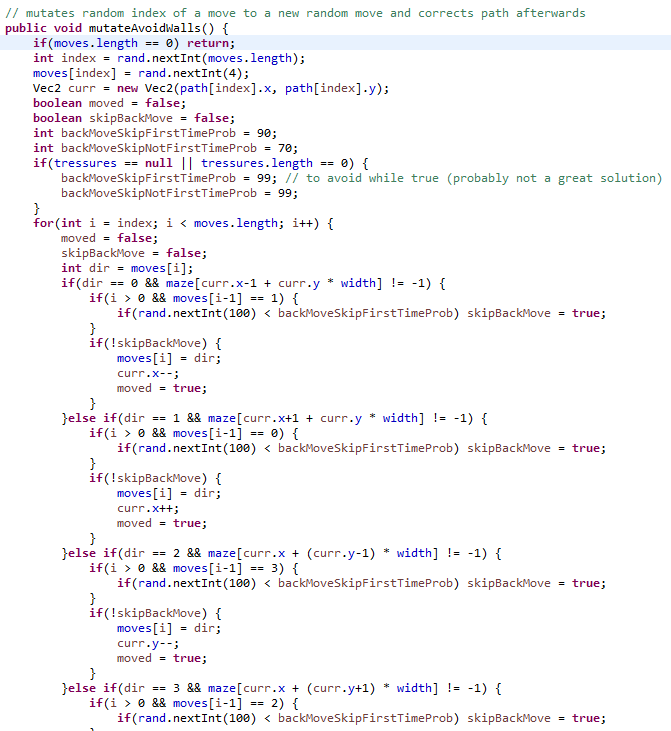
\includegraphics[scale=1]{randomMovePathCorrectionMutation1}
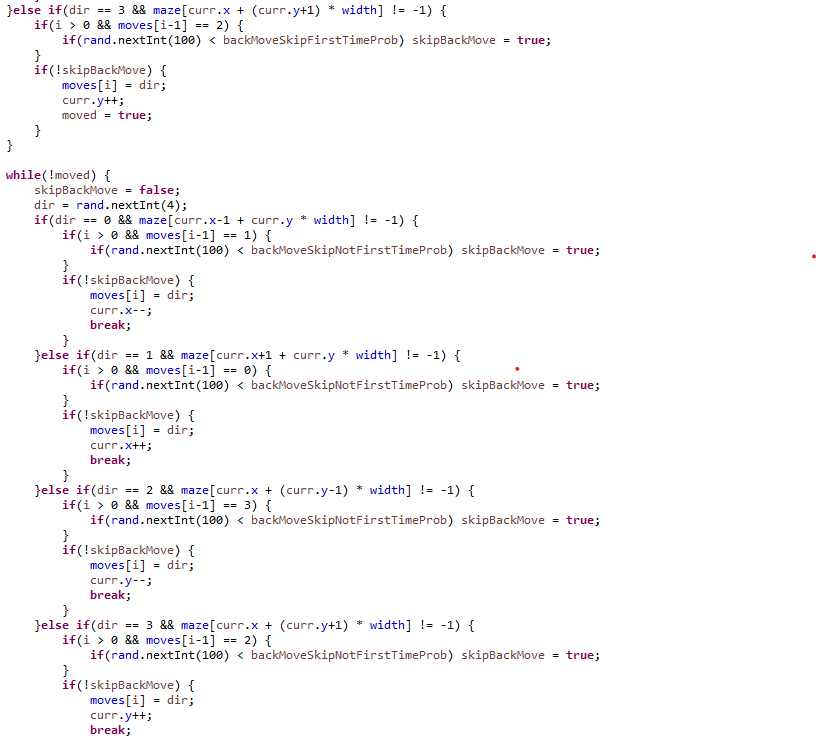
\includegraphics[scale=1]{randomMovePathCorrectionMutation2}
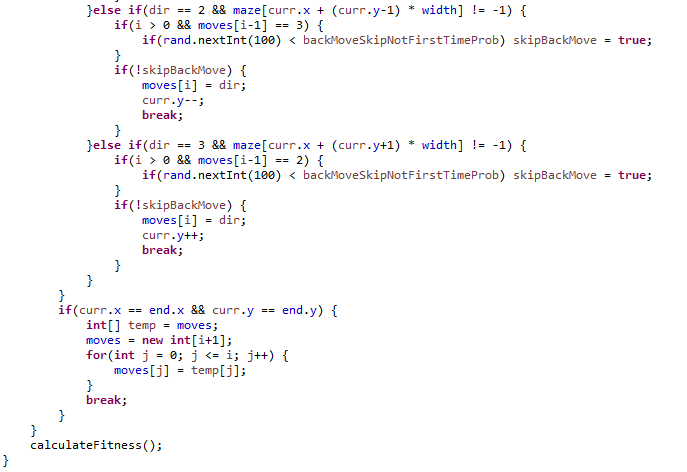
\includegraphics[scale=1]{randomMovePathCorrectionMutation3}

\subsubsection{Remove unneccesary moves}
Go through the path and check if the coordinate was already visited and no thresures were picked between visits. If that happens this part of the path
is useless so it should be removed:

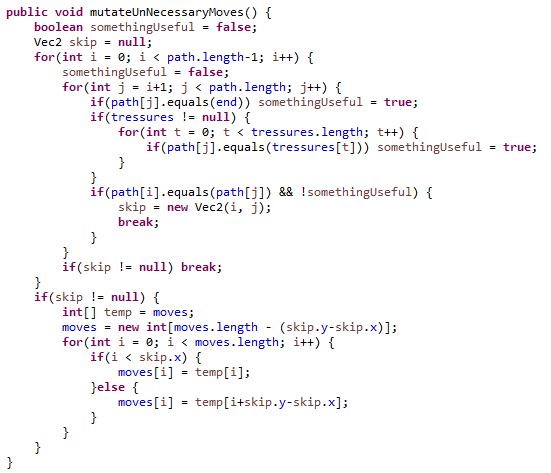
\includegraphics[scale=1]{removeUnNeccesaryMovesMutation}


\subsection{Generating initial population}
\subsubsection{Initial population of random paths}
Generates a random sequence of moves.

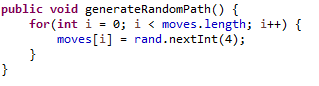
\includegraphics[scale=1]{generationRandomInitialPopulation}

\subsubsection{Initial population of random paths without going into walls}
Generates a random sequence of moves that doesn't go through walls.

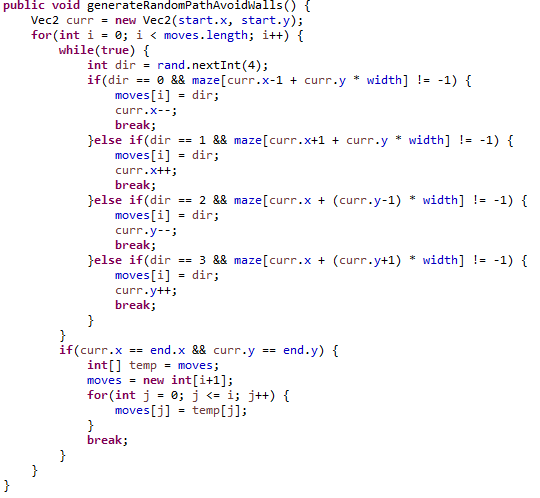
\includegraphics[scale=1]{generationRandomInitialPopulationAvoidWalls}

\section{Task 4 - Results}
Solutions of mazes:

\begin{center}

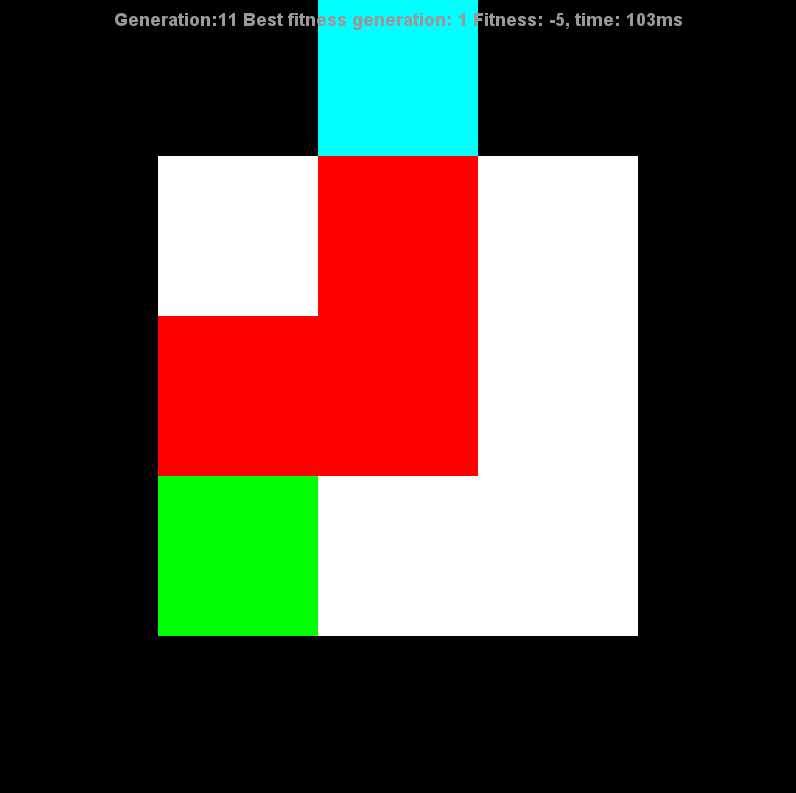
\includegraphics[scale=.6]{maze1}

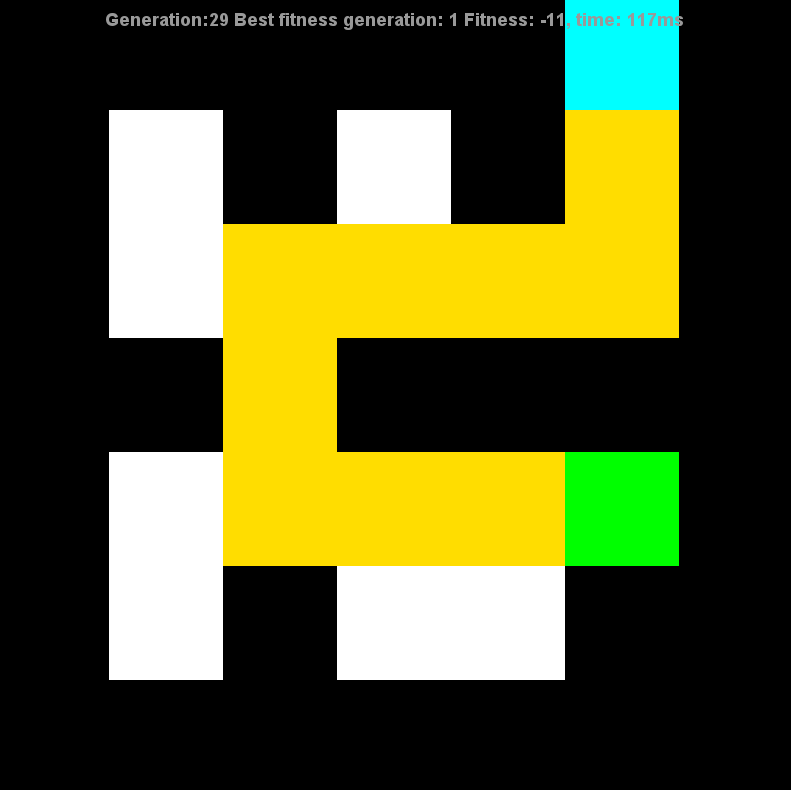
\includegraphics[scale=.6]{maze2}

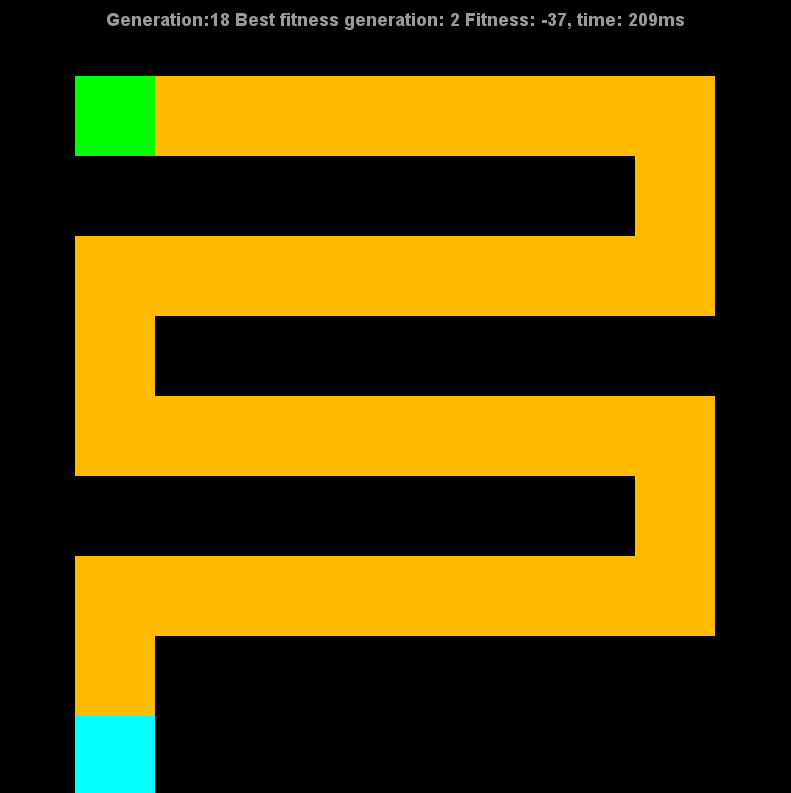
\includegraphics[scale=.6]{maze3}

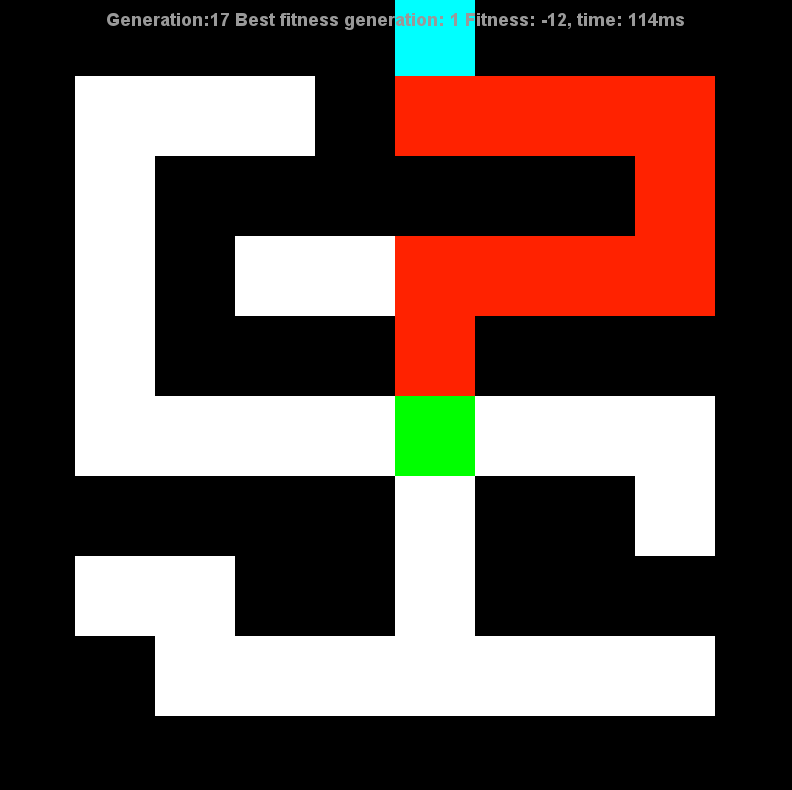
\includegraphics[scale=.6]{maze4}

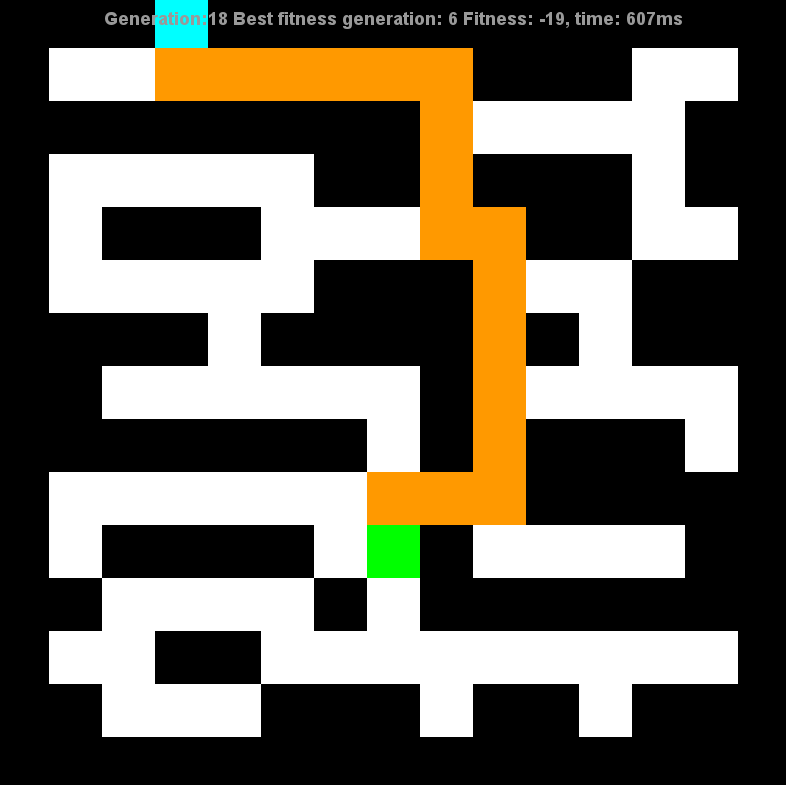
\includegraphics[scale=.6]{maze5}

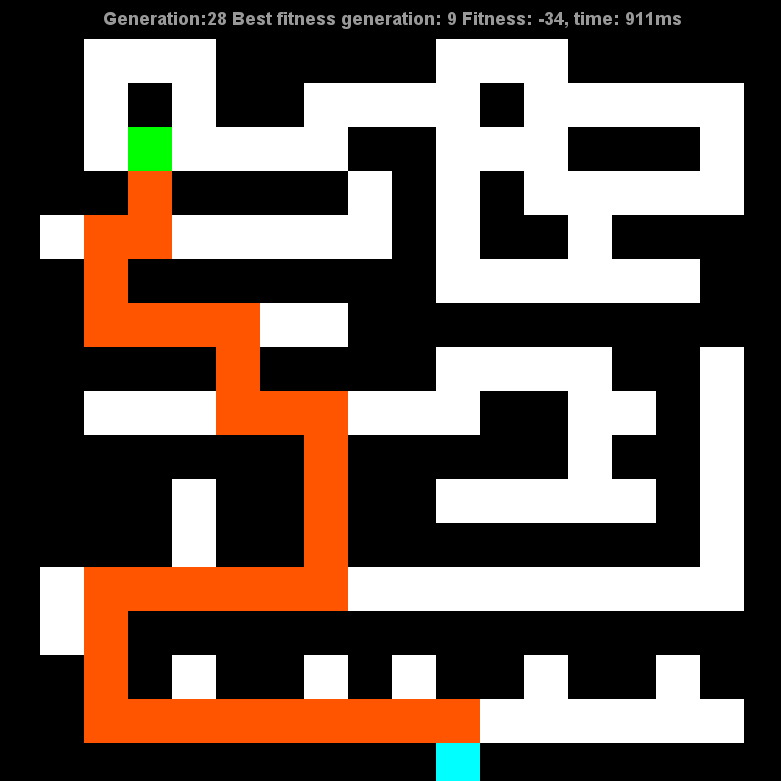
\includegraphics[scale=.6]{maze6}

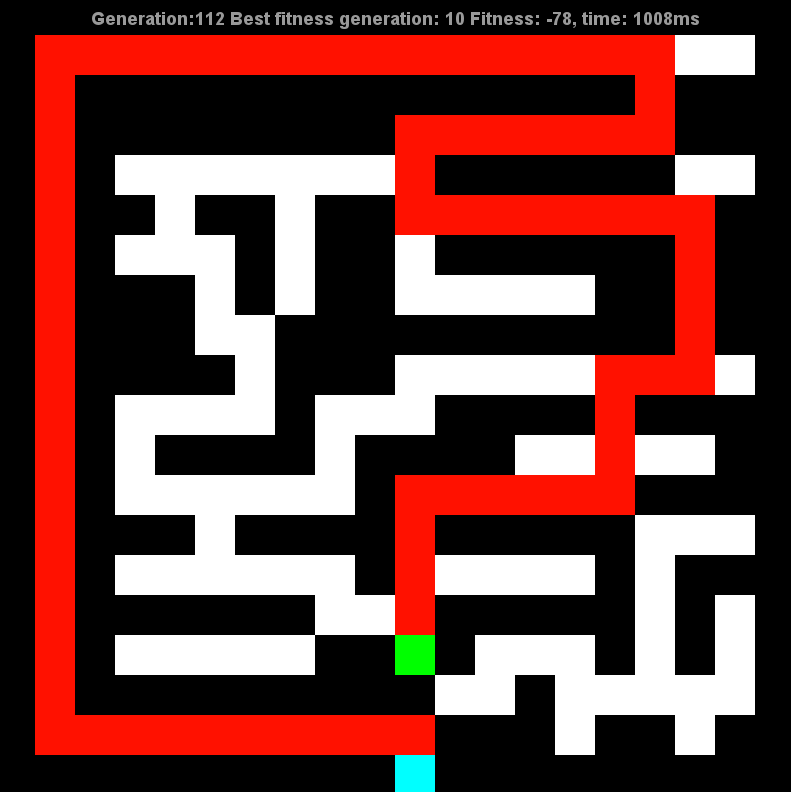
\includegraphics[scale=.6]{maze7}

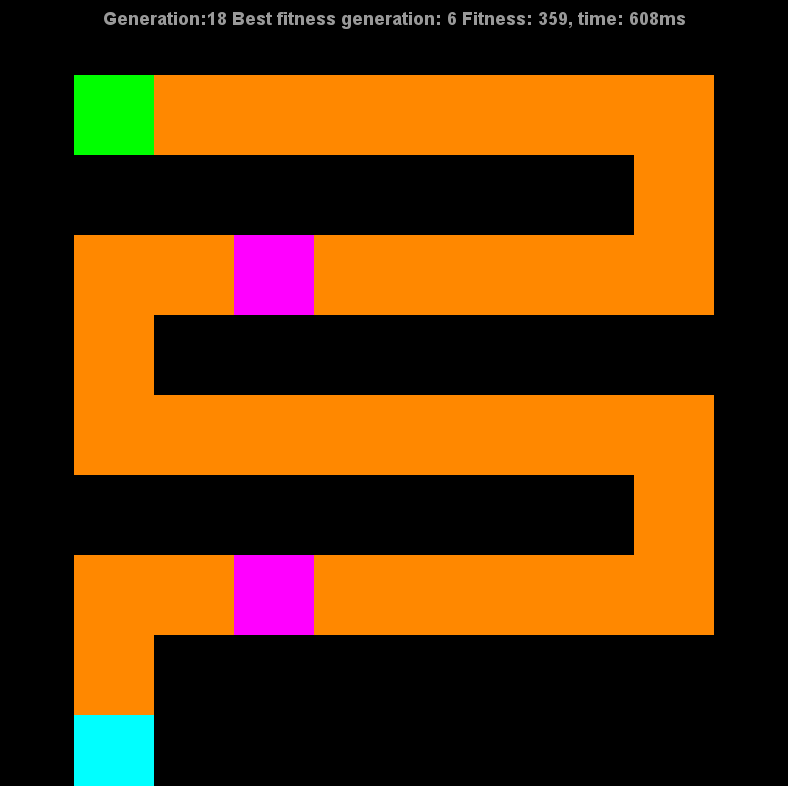
\includegraphics[scale=.6]{maze8}

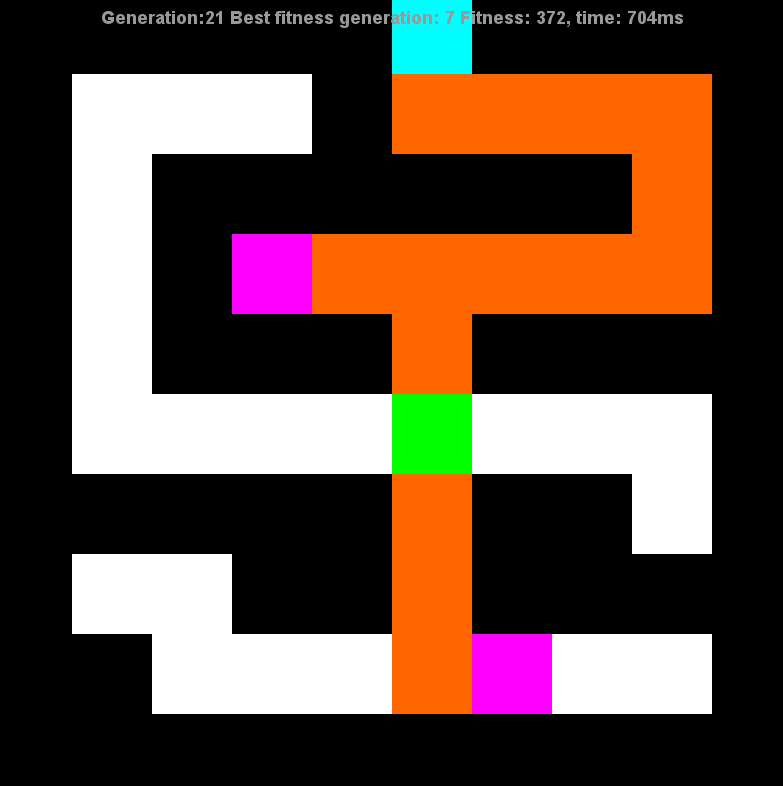
\includegraphics[scale=.6]{maze9}

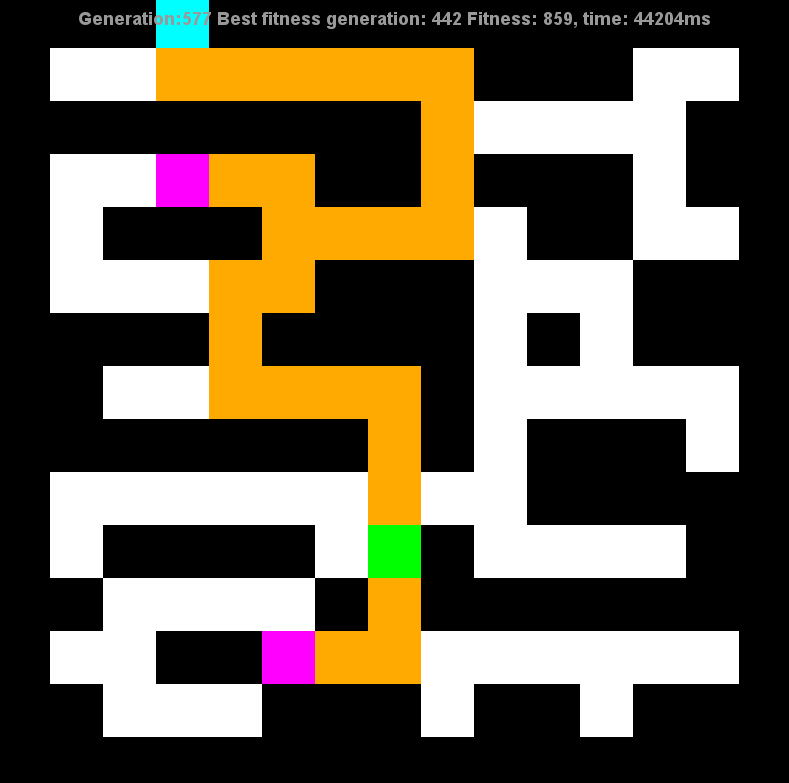
\includegraphics[scale=.6]{maze10}

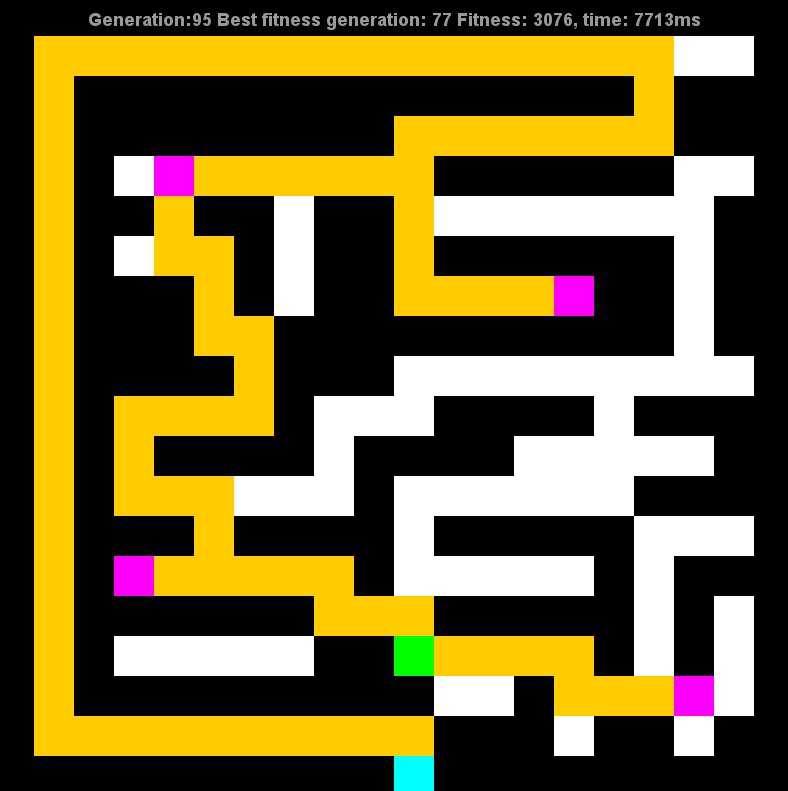
\includegraphics[scale=.6]{maze11}

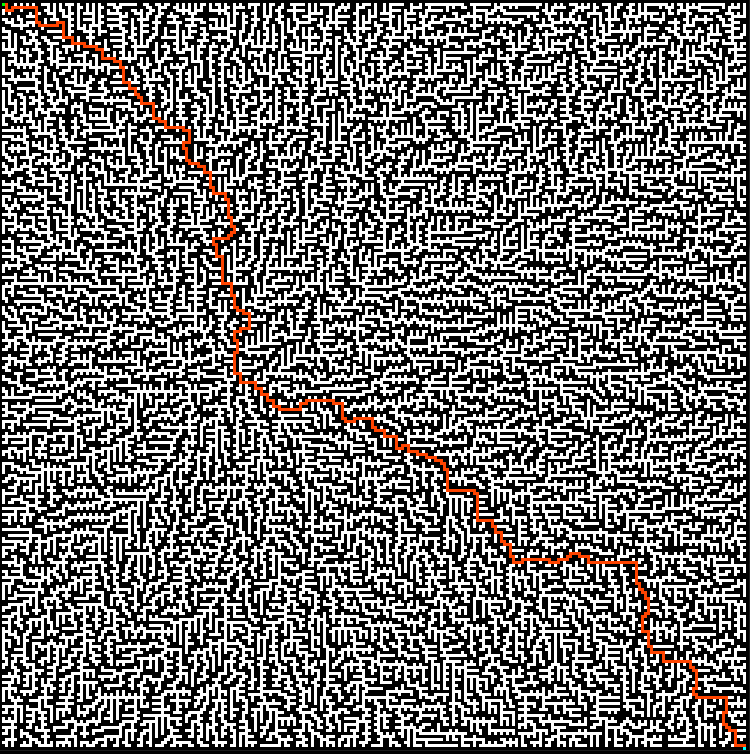
\includegraphics[scale=.6]{bigMaze}
\end{center}


\subsection{Performance comparison}
Selections: linearly biased selection works a lot better than a random selection.

Crossover: choosing a random parent works better than computing the intersections, because it is not computationaly expensive and mutations
can make this behaviour very well and fast.

Mutations: Combination of changing a random move along the path and then correcting next moves so that they don't go through walls woked best for us
with a mutation that removes unneccesary parts of the path (this mutation is only possible on chromosomes that make it to the end).

Initial population generation: Initial population generation should be generated randomly and should take walls into account, because in that way a big part
of a maze is searched in every generation (if mutations and crossovers have the same behaviour). Even better performance would be if back moves are less
likely.

Population size: We got the best results with initial population of size 1000. The number depends on the maze but bigger number means more of a maze will
be searched in first generation and thus the algorithm is more likely to converge faster. But too big number means every generation will be computed slower
so the "good" mutations will take more time to appear.

Elitism: 10 percent seems to be a good number. To small percentage might mean a very good candidate will get mutated and lost. Too big percentage will 
make algorithm slower and is not neccessary so it means we are wasting memory.

Mutation probability: 30 percent gave us a good results. We don't want to mutate with too big percentage because than all the data gained from genrations
will be lost. But too small of a percentage will make local maximums harder to avoid.

Back move probability: If a maze has no tresasures back moves should be avoided so the probability of back moves should be 0 (in our implementation
of the algorithm it is 1 percent so that we don't have to change the chromosome length when a dead end is found). If a maze contains tressures, we got very
good results with 10 percent probability to allow back move on a first try and 30 percent on every subsequent try.

Note: The results will vary and are hard to evaluate based on one try, because algorithm uses randomness.

\end{document}

















































